\documentclass[
  accentcolor=tud1c,	% Color theme for TUD corporate design
  colorbacktitle,		% Titlepage has colored background for title area
  inverttitle,			% Font color of title on titlepage is inverted
  german,				% Document is in english
  twoside
]{tudexercise}

\usepackage[ngerman]{babel}
\usepackage{units}
\usepackage[utf8]{inputenc}

\usepackage{listings}
\lstloadlanguages{C++}
\lstset{language=C++}
\lstset{captionpos=b}
\lstset{tabsize=3}
\lstset{breaklines=true}
\lstset{columns=flexible,keywordstyle=\color{red},stringstyle=\color{blue}}
\lstset{literate=%
{Ö}{{\"O}}1
{Ä}{{\"A}}1
{Ü}{{\"U}}1
{ß}{{\ss}}2
{ü}{{\"u}}1
{ä}{{\"a}}1
{ö}{{\"o}}1
}

\newcommand{\superscript}[1]{\ensuremath{^{\textrm{#1}}}}
\newcommand{\subscript}[1]{\ensuremath{_{\textrm{#1}}}}

\newcommand{\tag}{5}

\title{Übung zum\linebreak[1]C/C++-Praktikum\linebreak[1] Fachgebiet Echtzeitsysteme}
\subtitle{Übungen für den \tag{}. Tag}

\begin{document}

\begin{examheader}
	\textmb{Übung zum C/C++-Praktikum - Tag \tag{}}
\end{examheader}
\maketitle 


\section{Umgang mit den Mikrocontroller-Bords}

Die Entwicklung für den Mikrocontroller unterscheidet sich kaum von den bisherigen Übungen, da die Toolchain mit in Eclipse integriert ist. Der Programmcode wird in Eclipse in den Projekten, die für die einzelnen Aufgaben vorgesehen sind, geschrieben. Beim Starten des Build-Vorgangs wird zusätzlich zu den eigentlichen Kompilierungsschritten automatisch das Programm auf den Mikrocontroller übertragen und der Controller neu gestartet. Soll manuell das Programm neu gestartet werden, ohne ein neues Programm zu übertragen, hilft ein kurzer Druck auf den blauen Reset-Knopf.


\section{Systemtest}

Testen Sie das Zusammenspiel von Eclipse / Compiler / Flash auf Mikrocontroller, in dem Sie das vorgegebene Projekt p00\_flash bauen. Dies sollte am Schluss automatisch das Programm auf den angeschlossenen Mikrocontroller übertragen. Das Programm sollte auf der Sieben-Segment-Anzeige des Boards eine \textit{42} anzeigen.



\section{Embedded-Entwicklung}

Im Folgenden werden einzelne Hardwarekomponenten angesteuert. Dazu ist hier eine Übersicht über die auf dem Starterkit vorhandenen Komponenten gegeben.
\begin{center}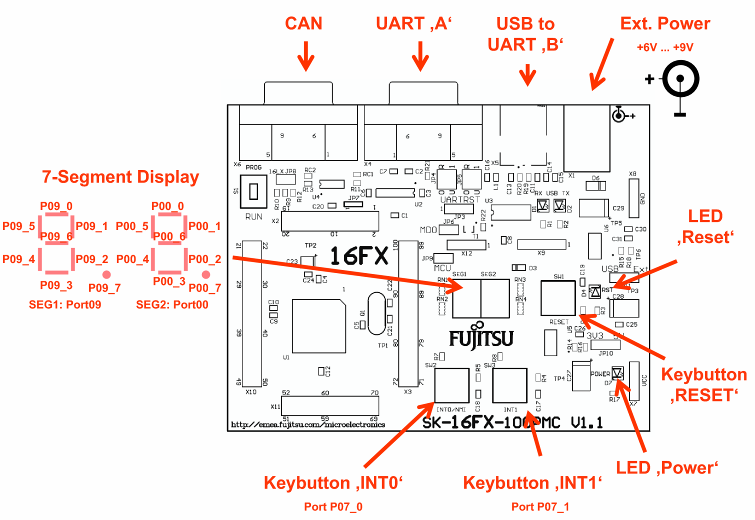
\includegraphics[width=0.7\textwidth]{starterkit}\end{center}

\subsection{p01\_7seg}
Implementieren Sie ein Programm, das die Zahlen 0 bis 99 auf den Sieben-Segment-Anzeigen ausgibt. Nach jeder Ausgabe einer Zahl soll eine Pause eingelegt werden.\\
Hinweise:\begin{itemize}
\item Für die Ausgabe der Zahlen 0 bis 9 steht Ihnen ein Array DEC7SEG zur Verfügung, welches die benötigten Were für die Ports für die jeweiligen Ziffern enthält.
\item Die Pause kann durch eine Schleife produziert werden, die in jedem Zyklus den Befehl \texttt{\_\_wait\_nop()} aufruft. Eine Konstante DELAY steht Ihnen zur Verfügung für die Anzahl der Schleifendurchläufe. Achten Sie insbesondere darauf, dass Sie hier den Datentyp long verwenden müssen!
\item Die beiden Anzeigen sind an den Ports 09 und 00 angeschlossen. Die Ansteuerung erfolgt logisch invertiert, das bedeutet wenn ein Ausgang für ein Segment logisch 0 ist leuchtet dieses, bei 1 ist es aus.
\item Beispiel: ein \glqq{}E\grqq{} kann durch das Setzen der Pins 0, 3, 4, 5 und 6 auf low gezeichnet werden. Binär: 10000110, Hexadezimal: 0x86
\end{itemize}
\begin{center}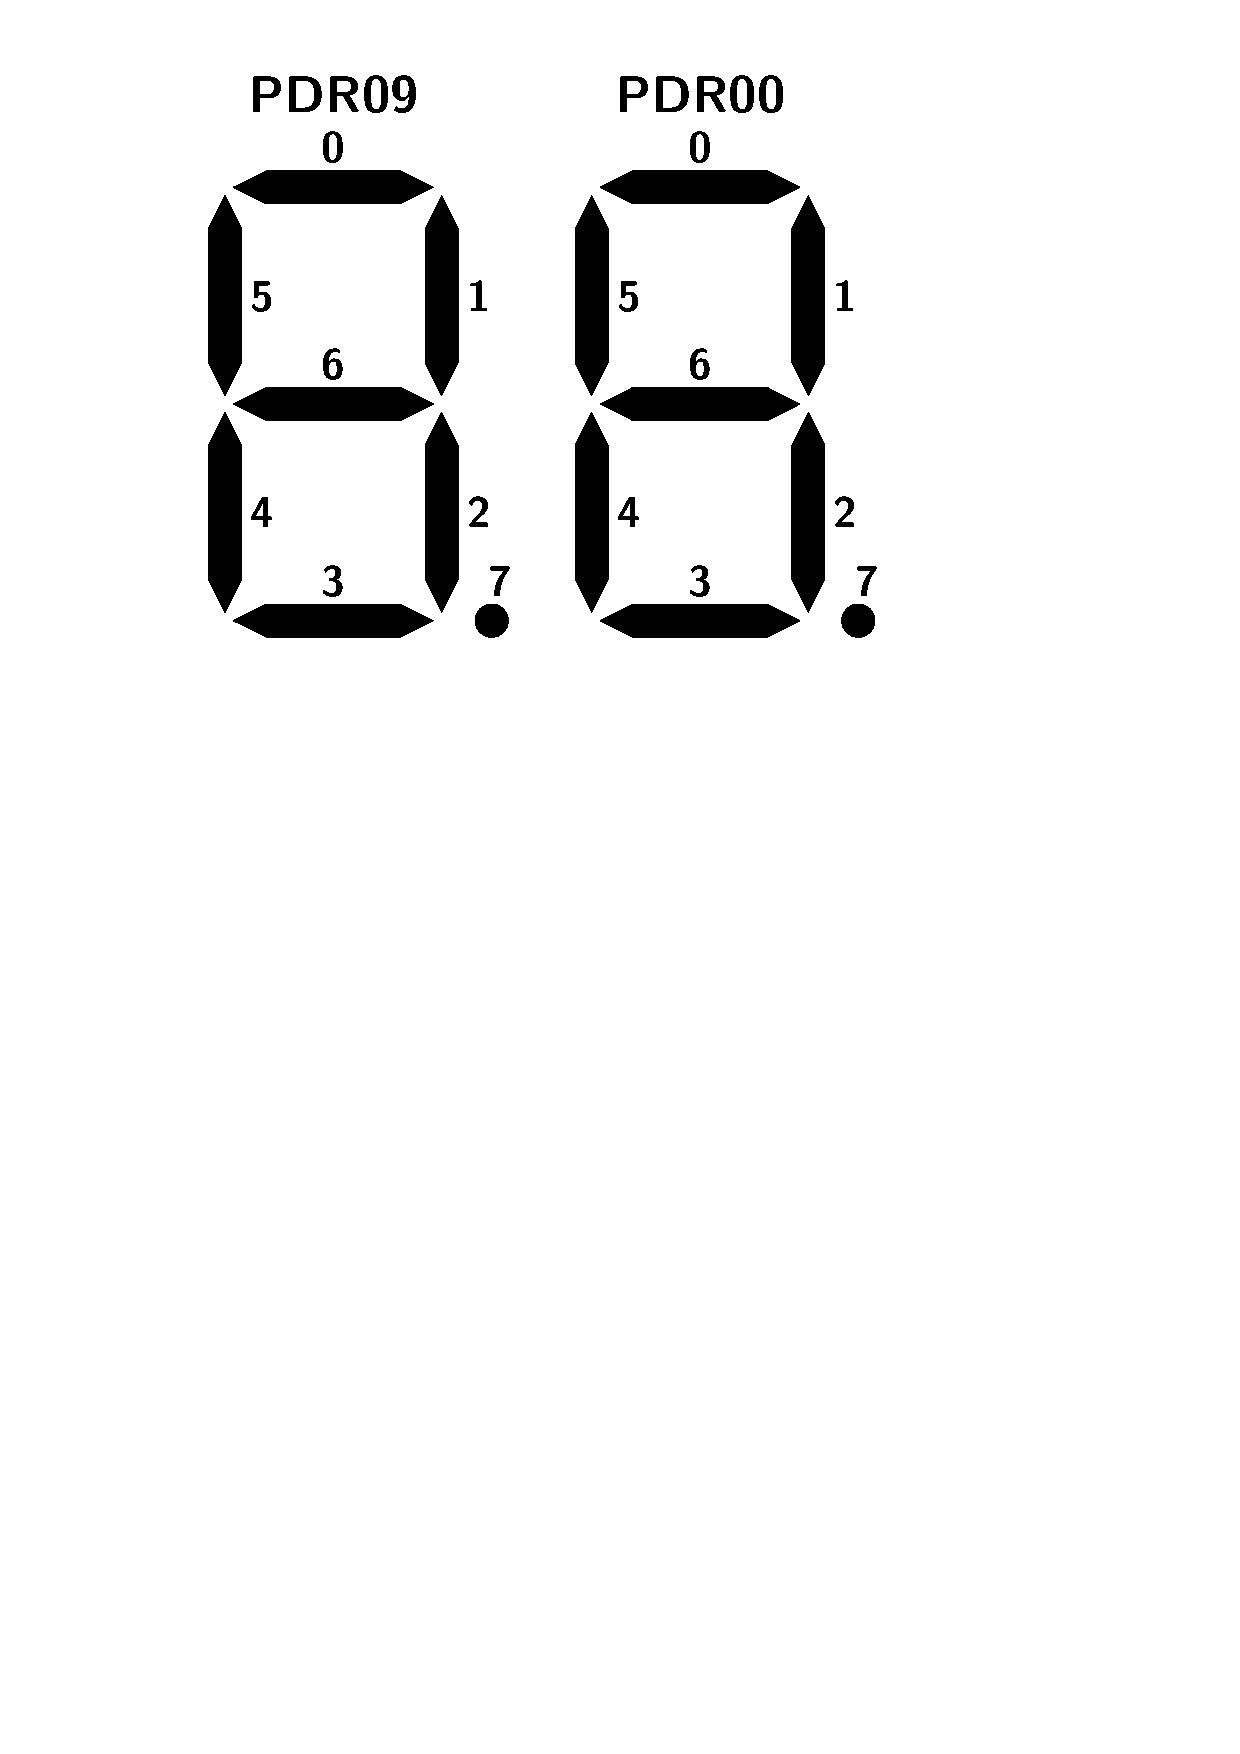
\includegraphics[width=0.3\textwidth]{7seg}\end{center}

\subsection{p02\_buttons}
Erstellen Sie einen Counter. Das Programm soll zu Beginn den Wert 0 anzeigen. Bei Druck auf die rechte Taste soll der Wert erhöht, bei Druck auf die linke Taste erniedrigt werden. Wird 99 angezeigt und die rechte Taste gedrückt, soll der Counter auf 0 gesetzt werden. Umgekehrt ebenso (counter==0, linke Taste gedrückt $\Rightarrow$ counter=99).\\
Hinweise:\begin{itemize}
\item Ein Button ist üblicherweise für mehrere tausend CPU-Zyklen gedrückt!
\item Ein Tastendruck ist durch den Übergang von high auf low definiert. Da in jedem Zyklus nur der aktuell Wert abgefragt werden kann, müssen Sie den aktuellen Wert mit einem gespeicherten Wert aus dem vorigen Durchlauf vergleichen.
\item Der linke Taster ist an Port 07 Pin 0, der rechte an Pin 1 angeschlossen. Bei gedrücktem Taster liegt ein Low-Pegel am Eingang, sonst ein High-Pegel.
\end{itemize}

\subsection{p03\_util}
Wie in Aufgabenteil a) sollen hier die Zahlen 0 bis 99 ausgegeben werden, aber unter der Verwendung von eigens dafür geschriebenen Funktionen:
\begin{lstlisting}
void wait(long w)          // für w Zyklen pausieren
void setLeft7Seg(int i)    // Zahl i auf linker Anzeige ausgeben falls i im gültigen Bereich (0 bis 9)
void setRight7Seg(int i)   // ebenso wie eben, nur für die rechte Anzeige
void set7Seg(int i)        // Zahl (0 bis 99) auf 7-Segment-Anzeigen darstellen
\end{lstlisting}

\subsection{p04\_adc}
Schreiben Sie ein Programm, das den Spannungswert von AN1 (linker Schieberegler) auf der linken Sieben-Segment-Anzeige und den Spannungswert von AN2 (rechter Schieberegler) auf der rechten Sieben-Segment-Anzeige ausgibt. Skalieren Sie dazu den resultierenden Wertebereich von 0 bis 255 auf 0 bis 9.\\
Hinweise:
\begin{itemize}
\item Einige Funktionen aus Aufgabenteil c) können hier eingesetzt werden.
\item Achten Sie auf die richtige Initialisierung von \textit{ADER0}.
\item Der Wert für \textit{ADSR} besteht aus 16 Bits (0110 11xx xxxy yyyy\textsubscript{b}), wobei xxxxx für den Startkanal der Konvertierung und yyyyy für den Endkanal steht. Für unsere Zwecke nehmen diese beiden 5\,Bit Blöcke immer entweder 00001 (AN1) oder 00010 (AN2) an.
\item Lesen Sie die beiden Werte nacheinander aus, verwenden Sie also immer die gleiche Zahl für Start- und Endkanal während einer Konvertierung.
\end{itemize}

\subsection{p05\_lcdbasics}
Ziel dieser Aufgabe ist es, die linke Seite des Displays anzusteuern und alle Zellen mit dem Wert aa\textsubscript{h} (10101010\textsubscript{b}) zu belegen.\\
Hinweise:
\begin{itemize}
\item Für diese Aufgabe benötigen Sie die Dokumentation des Displays (\textit{Display\_AV128641YFBY-WSV\#.pdf}), dort insbesondere den Abschnitt mit den Befehlen (Setzen der x- und y-Adresse, \textbf{Einschalten des Displays}, Senden der Daten).
\item Achten Sie darauf, dass Sie nach jedem Befehl (Daten oder Instruktion) das Enable-Signal an das Display senden. Es empfiehlt sich, eine Funktion \textit{void lcd\_sendEnable(void)} zu implementieren, die den Enable-Pin auf 1 setzt, kurz wartet und dann wieder auf 0 setzt und erneut kurz wartet. Verwenden Sie als Warteintervall die Konstante LCD\_T. Denken Sie daran, das Enable-Pin zu Beginn des Programms mit 0 zu initialisieren.
\item Das Display ist logisch aufgeteilt in zwei Hälften zu je 64 x 64 Pixel (siehe untenstehende Graphik). Welche Hälfte einen Befehl verarbeiten soll wird ausgewählt, in dem deren Chip-Select-Signal CS1 bzw. CS2 auf 1 gesetzt wird, das andere auf 0.

\item Die Ansteuerung erfolgt über Pins mit festgelegten Funktionen. Zur Vereinfachung wurden bereits im Projekt für diese Aufgabe Definitionen vorgegeben, so dass die Pins über einfache Namen angesteuert werden können. Die Namen entsprechen den Pins, wie sie im Datenblatt ab Seite 10 zu finden sind.

\begin{center}
\begin{tabular}{l|l|l}
Name & Funktion & Controllerpin/port \\ 
\hline 
LCD\_PORT\_DB & Datenbus (DB0 - DB7) & P01 \\ 
LCD\_PIN\_DI & Data (1) / Instruction (0) & P02\_0 \\ 
LCD\_PIN\_RW & Read (1) / Write (0) & P02\_1 \\ 
LCD\_PIN\_E & Enable & P02\_2 \\ 
LCD\_PIN\_CS1 & Linker Chip (1 = aktiv) & P02\_3 \\ 
LCD\_PIN\_CS2 & Rechter Chip (1 = aktiv) & P02\_4 \\ 
LCD\_PIN\_RESET & Reset-Signal (0 = aktiv) & P02\_5 \\ 
\end{tabular}
\end{center}

\item Grundsätzliches Prinzip zum Senden von Befehlen:\begin{enumerate}
\item Daten am Datenbus bereitstellen: PORT\_DB, PIN\_DI, PIN\_RW wie gewünscht setzen, ein Chip-Select (PIN\_CS1 oder PIN\_CS2) aktivieren
\item Enable-Signal schicken (=> high => low)
\end{enumerate}
Beachten Sie: Das Reset-Signal muss immer 1 (deaktiviert) sein.

\item Vorgehen zum Schreiben von Bilddaten:\begin{enumerate}
\item Setzen der x-Adresse (Zeilenblock)
\item Setzen der y-Adresse (Spalte)
\item Senden von 8 Bit Daten (eine \glqq{}Zelle\grqq{} von 8 Pixeln Höhe)
\end{enumerate}
Vereinfachung: Der \textit{y}-Zähler wird nach dem Senden von Daten im Display automatisch hochgezählt. Somit kann \textit{y} zu Beginn jeder Zeile auf 0 gesetzt werden und muss danach für den Rest der Zeile nicht mehr manuell gesetzt werden.

\begin{center}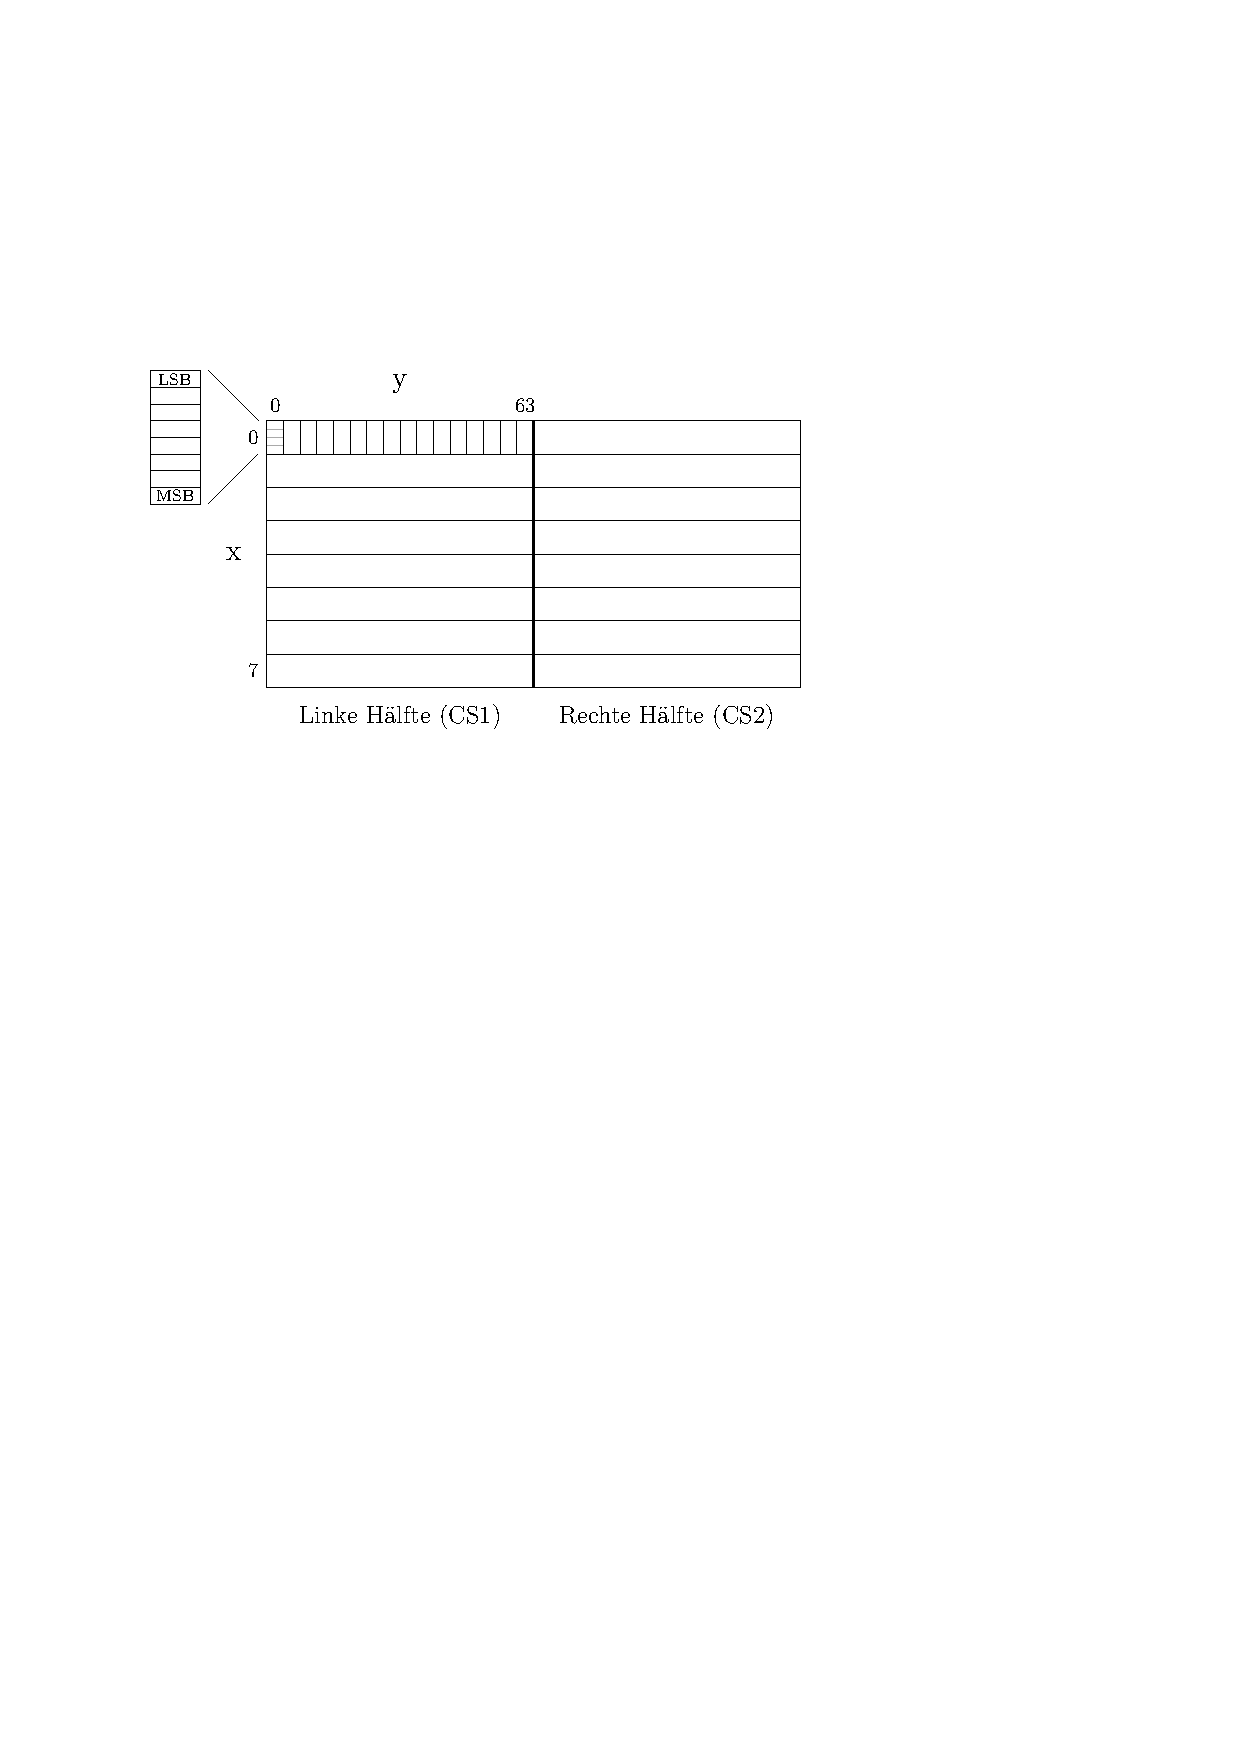
\includegraphics[width=0.6\textwidth]{display_aufbau}\end{center}


\end{itemize}

\subsection{p06\_lcd}
Nun soll das Display wie ein Bildschirm angesteuert werden können. Es gibt einen Buffer \textit{lcd\_buffer}, auf dem Pixeloperationen durchgeführt werden sollen. Schreiben Sie folgende Funktionen:
\begin{lstlisting}
void lcd_clear()                             // Löscht den Buffer (setzt alle Werte im Buffer auf 0).
void lcd_drawPixel(int x, int y, int black)  // Setzt einen Pixel an Position (x,y) wenn black == 1 ist,
                                             // bei black == 0 wird der Pixel an Position (x,y) gelöscht.
                                             // Keine Operation bei ungültigen Werten für x, y oder black.
void lcd_flush()                             // Gibt den Buffer an das Display aus.
\end{lstlisting}
Hinweise:
\begin{itemize}
\item Ein Testprogramm steht bereits zur Verfügung, welches ein Schachbrettmuster auf dem Display ausgibt -- wenn Ihre Funktionen komplett und korrekt implementiert sind.
\item Achten Sie auch hier darauf, dass das Display zunächst per Befehl eingeschaltet werden muss.
\item Für die Funktion \textit{lcd\_drawPixel} werden Bitoperationen benötigt. Eine Skizze kann hier sinnvoll sein, um sich vorzustellen, wie die Bitoperationen arbeiten.
\end{itemize}


\end{document}
